\documentclass[11pt,a4paper]{article}
\usepackage[margin=2.3cm]{geometry}
\usepackage{amsmath,amssymb,booktabs,tabularx,xcolor,hyperref,enumitem}
\usepackage{tikz}
\usetikzlibrary{positioning,arrows.meta,fit}
\hypersetup{colorlinks,linkcolor=blue!50!black,urlcolor=blue!50!black}
\setlist{itemsep=2pt,topsep=3pt}
\newcommand{\code}[1]{\texttt{\small #1}}
\newcommand{\why}[1]{\par\noindent\textcolor{teal!60!black}{\textit{Intuition:} #1}\par}
\definecolor{inp}{HTML}{4E79A7}\definecolor{lay}{HTML}{59A14F}\definecolor{out}{HTML}{E15759}

\title{HY Analyst: from method to code\\[2pt]\large How the high yield mispricing method works, and where each part lives in \code{hy/}}
\author{FundamentalQuantmental}
\date{21 October 2026}

\begin{document}
\maketitle

\section*{The method in one page}

\textbf{The question.} Which high yield bonds pay more spread than their risk justifies?

\textbf{The answer in four moves.}
\begin{enumerate}
\item Measure the issuer today: earnings, cash, debt, and risk flags (Section~\ref{sec:state}).
\item Project the issuer forward under named scenarios. Let the macro forecast set how likely each scenario is (Section~\ref{sec:forward}).
\item Turn the projections into a probability of default and a loss given default. Their product, scaled by the market price of risk, is the \emph{anchor spread}. A second model explains what the anchor misses (Sections~\ref{sec:recovery} and~\ref{sec:fair}).
\item Compare the market spread with the fair spread. A bond is cheap only when it sits outside a band that measures the model's own error (Section~\ref{sec:fair}). Seven signals and an event risk model turn that gap into positions (Sections~\ref{sec:signals} and~\ref{sec:events}).
\end{enumerate}

\textbf{The base.} Gatto, \emph{The Credit Investor's Handbook} (Wiley, 2023), gives the analyst process. The book has no statistical models. This system keeps the book's process as the feature set and adds the models around it. \code{docs/methodology.md} is the full specification; its section numbers match the module docstrings.

\textbf{The rule that protects every result.} Every input carries two dates: \code{as\_of} (the period it describes) and \code{available\_at} (the first moment the market could read it). A model reads only fields available before the decision time. A test enforces this.

\begin{figure}[h]
\centering
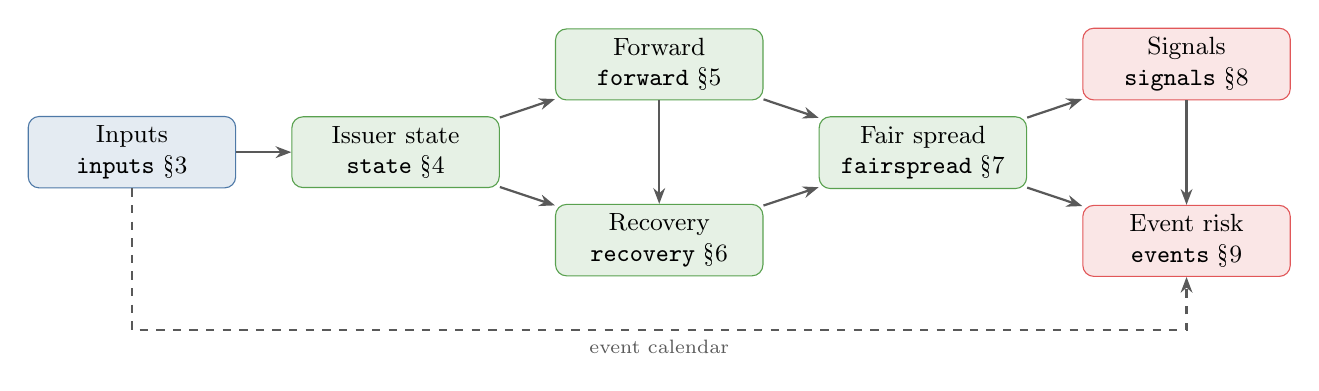
\begin{tikzpicture}[
  node distance=5mm and 7mm,
  box/.style={draw,rounded corners,align=center,font=\small,minimum height=8mm,text width=24mm},
  i/.style={box,fill=inp!15,draw=inp}, l/.style={box,fill=lay!15,draw=lay}, o/.style={box,fill=out!15,draw=out},
  a/.style={-{Stealth[length=2mm]},thick,gray!70!black}]
\node[i] (in) {Inputs\\\code{inputs} \S3};
\node[l,right=of in] (st) {Issuer state\\\code{state} \S4};
\node[l,above right=2mm and 7mm of st] (fw) {Forward\\\code{forward} \S5};
\node[l,below right=2mm and 7mm of st] (rc) {Recovery\\\code{recovery} \S6};
\node[l,below right=2mm and 7mm of fw] (fs) {Fair spread\\\code{fairspread} \S7};
\node[o,above right=2mm and 7mm of fs] (sg) {Signals\\\code{signals} \S8};
\node[o,below right=2mm and 7mm of fs] (ev) {Event risk\\\code{events} \S9};
\draw[a] (in)--(st); \draw[a] (st)--(fw); \draw[a] (st)--(rc); \draw[a] (fw)--(rc);
\draw[a] (fw)--(fs); \draw[a] (rc)--(fs); \draw[a] (fs)--(sg); \draw[a] (fs)--(ev); \draw[a] (sg)--(ev);
\draw[a,dashed] (in.south) |- ++(0,-18mm) -| (ev.south) node[pos=0.25,below,font=\scriptsize]{event calendar};
\end{tikzpicture}
\caption{One spine, two consumers. Blue: data. Green: models. Red: what the desk uses. Every table written by the pipeline follows the schemas in \code{outputs} (\S10).}
\end{figure}

\section*{What this means for you}
\begin{itemize}
\item \textbf{The code runs end to end on synthetic data today.} From the repository root run\\ \code{PYTHONPATH=. python3 scripts/demo\_pipeline.py}.\\ It takes one synthetic universe through Sections 5 to 8 and prints a force rank.
\item \textbf{The code has not seen real data yet.} The real-data step is to load filings, TRACE prices and macro series into the \code{inputs} records. Your \code{marketdb} has TRACE but not issuer financials with release dates.
\item \textbf{Each claim in the method is now a test.} Section~\ref{sec:tests} lists them. A green test means the formula does what the method says. It does not yet mean the signal makes money.
\end{itemize}

\newpage
\section{Inputs and the look-ahead guard (\S3, \code{hy/inputs.py})}
\label{sec:inputs}
\textbf{Book.} The analyst reads the 10-K, the indenture, and the market (Chapters 3, 5, 12).

\textbf{Code.} Each record type (\code{IssuerFinancials}, \code{Tranche}, \code{Event}) inherits \code{Stamped}, which holds \code{key}, \code{as\_of} and \code{available\_at}. \code{PointInTimeStore.view(t)} returns the latest version of each record that the market could see at time $t$. A restatement is a new version of the same key with a later \code{available\_at}; it replaces the original only after its own release.
\why{a backtest that reads a restated number before the restatement date finds alpha that never existed.}

\section{Issuer state (\S4, \code{hy/state.py})}
\label{sec:state}
\textbf{Book.} Steps 2 and 3: qualitative risks, profitability, cash flow, capital structure (Chapters 6--9).

\textbf{Adjusted EBITDA.} Add back only items that do not recur:
\[ EBITDA^{adj}_t = EBITDA^{rep}_t + \textstyle\sum_i a_i\,NR_{i,t},\qquad a_i\in\{0,1\}. \]
\why{a ``one-off'' charge that comes every year is an operating cost.}

\textbf{Free cash flow.} The code charges the cash part of each add-back:
\[ FCF_t = EBITDA^{adj}_t - CashNR_t - Capex_t - CashInterest_t - CashTax_t - \Delta WC_t. \]
\why{an add-back for a cash restructuring charge raises earnings but not cash.} \code{methodology.md} \S4.2 adopted this on 21 October 2026.

\textbf{Leverage through the tranche.} Senior claims at face, the tranche under analysis at market:
\[ Lev^{face}_k=\frac{\sum_{rank_j\le rank_k}F_j}{EBITDA^{adj}},\qquad Lev^{mkt}_k=\frac{\sum_{rank_j<rank_k}F_j+P_kF_k}{EBITDA^{adj}}. \]
\why{$Lev^{mkt}_k$ is the creation multiple: the company value at which a buyer of this bond owns the business.}

\textbf{Covenant headroom.} $H_t = 1-Lev^{cov}_t/Lev^{max}_t$. At origination lenders set $Lev^{max}=D/((1-c)\,EBITDA^{mgmt})$; a 15\% cushion on a 4.0x plan gives 4.7x (p.~356).

\textbf{Rating gap.} An ordinal model predicts the rating from scale, leverage, coverage, margin and sector. Fitted rating minus agency rating, in notches, is the gap.
\why{ratings lag prices (p.~274), so a bond rated above its fundamentals is a downgrade candidate.}

\section{Forward estimates (\S5, \code{hy/forward.py})}
\label{sec:forward}
\textbf{Book.} Build management, base and downside cases; assign probabilities by judgement (Chapter 10).

\textbf{Scenario engine.} For scenario $s$ and quarter $h$:
\begin{align*} Rev^s_h&=Rev^s_{h-1}(1+g^s_h),\qquad EBITDA^s_h=Rev^s_h(1-v^s_h-a^s_h),\\ FCF^s_h&=EBITDA^s_h-Capex^s_h-i_h(m)D^s_{h-1}-Tax^s_h-\Delta WC^s_h. \end{align*}
Negative FCF draws the revolver. Interest uses last quarter's debt, so the engine needs no circular solver.
\why{liquidity and leverage come out of one recursion, so they cannot contradict each other.}

\textbf{Macro sets the weights.} A pooled logistic model gives the chance of a large EBITDA fall in the next four quarters:
\[ P(EBITDA_{t+4}<(1-\delta_i)EBITDA_t\mid m_t,sector_i)=\sigma(\theta_0+\theta^\top m_t+\theta_{sector}). \]
That probability is the weight of the moderate downside. The severe case takes a fixed fraction of it, and the base case takes the rest.
\why{in a late cycle every issuer's downside weight rises before any issuer misses.}

\textbf{Forward features.} Weighted mean and spread of leverage at 4 and 8 quarters, the peak downside leverage, the minimum downside liquidity, and the probabilities of covenant breach, cash shortfall and failed refinance. The book's own check (p.~311) is the flag $w_{down}>0.5$: then the downside should be the base case.

\section{Valuation and recovery (\S6, \code{hy/recovery.py})}
\label{sec:recovery}
\textbf{Book.} Four valuation methods (Chapter 11), priority of claims (Chapter 9), and documents that move claims ahead of yours (Chapter 18).

\textbf{Value as a distribution.} $\log V\sim N(\mu_V,\sigma_V^2)$, $\mu_V=\log V_{mid}$, $\sigma_V=(\log V_{high}-\log V_{low})/(2\times1.28)$.
\why{the low and high ends of the football field are read as the 10th and 90th percentiles.}

\textbf{Waterfall.} Tranche $k$ owns the slice of value between $S_k$ (all claims ahead) and $S_k+F_k$:
\[ Pay_k(V)=\min\big(F_k,\max(0,V-S_k)\big),\qquad R_k=E[Pay_k(V)]/F_k. \]
This is a call spread on firm value. With lognormal $V$ it has a closed form, so the code needs no simulation; a Monte Carlo check confirms it.

\textbf{Liability management.} $R^{adj}_k=(1-\pi_{LME})R_k+\pi_{LME}R^{LME}_k$. The probability $\pi_{LME}$ rises with loose baskets, a bare-majority amendment vote, sponsor history, and closeness to distress.
\why{after the Serta-style uptier, PU Corp recovery fell from 70--82.5\% to 24.8--49.9\% (pp.~503--504).}

\section{Fair spread and mispricing (\S7, \code{hy/fairspread.py})}
\label{sec:fair}
\textbf{Book.} Risk is probability of default times loss given default (p.~119). The book compares bonds by judgement; it has no spread model.

\textbf{Anchor.} $\lambda_i=-\log(1-PD^{12m}_i)$, $s^{EL}_i=\lambda_iLGD^{adj}_i$, $s^{anchor}_{i,t}=\kappa_t\,s^{EL}_i$. The PD model is calibrated so that its mean by rating matches the agency default table.
\why{$\kappa_t$ is the market price of credit risk: high after a sell-off, low in a frothy market.}

\textbf{Second stage.} $\log s_{i,t}=\log s^{anchor}_{i,t}+f_t(x_{i,t})+\eta_{sector,t}+\varepsilon_{i,t}$. The model $f_t$ is a gradient-boosted tree with monotone constraints: the spread must rise with leverage and fall with coverage.
\why{the constraints stop the model from learning a wrong sign, so a large residual is never a sign error.}

\textbf{The band.} $z=\varepsilon/\hat\sigma(x)$. Split conformal prediction, run separately in each rating and liquidity cell, gives a threshold $q_{1-\alpha}$. A bond is cheap when $z>q_{1-\alpha}$. Adaptive conformal inference moves $\alpha_t$ so that coverage stays on target as spreads drift.
\why{illiquid CCC bonds are noisy; the band is wider there, so the model does not call noise ``cheap''.}

\textbf{Convergence.} An AR(1) on each residual gives the half-life $\log2/(-\log\rho)$ and the expected return $carry_h+D^s(1-\rho^h)m$.

\section{Signals (\S8, \code{hy/signals.py})}
\label{sec:signals}
\begin{tabularx}{\linewidth}{@{}lXl@{}}\toprule
Signal & What it buys & Main failure \\\midrule
S1 residual & Spread above the conformal band & Fact the model misses \\
S2 momentum & Fundamentals improved more than the spread & Non-cash improvement \\
S3 revision & Forward leverage falls; analyst below consensus & Analyst bias \\
S4 capital structure & Tranche gap above the recovery gap & Both legs go to recovery \\
S5 documents & In-the-money change-of-control put; protected tranche & Fall-away clause \\
S6 ratings & Positive rating gap, before the upgrade & Already priced \\
S7 sector & Sector cheap to its macro forecast & Stale forecast \\\bottomrule
\end{tabularx}

\medskip
The composite weights each signal by its trailing rank IC in the current cycle phase; a signal with negative IC gets zero weight. The composite is made neutral to index beta and duration. The force rank sorts the whole universe, not each sector (p.~369). No position enters without \code{replaces\_position}.

\section{Event risk (\S9, \code{hy/events.py})}
\label{sec:events}
A dated event (earnings, covenant test, maturity, rating review, LME) has a set of outcomes. A macro forecast is four to six named paths. For each outcome $o$ and path $m$ the code changes the features and re-evaluates the fair spread:
\[ \Delta P_i(o,m)\approx-D_i\Delta y(m)-D^s_i\big[\Delta s^{sys}(m)+\hat s_i(x_i(o,m))-\hat s_i(x_i)\big]+carry_h-\mathbb 1\{default\}(P_i-100R^{adj}_i). \]
\why{the model that says a bond is cheap also says how much it loses on a miss.}

\textbf{Why yields need a split.} $\Delta s^{sys}=\beta_g\Delta y^{growth}+\beta_p\Delta y^{policy}$ with $\beta_g<0$, $\beta_p>0$. Yields up on strong growth tighten spreads; yields up on Fed tightening widen them. So a high yield bond has a short effective rate duration in a growth move and a long one in a policy move.

\textbf{Pair trades.} Size pairs by jump-to-default, not DV01: $N_j/N_k=(P_k-100R_k)/(P_j-100R_j)$. In a filing both legs converge to recovery (p.~530).

\section{What the tests prove}
\label{sec:tests}
Run \code{python3 -m pytest} from the repository root. On 21 October 2026, 118 tests passed in about 5 seconds.

\medskip
{\small\begin{tabularx}{\linewidth}{@{}llrX@{}}\toprule
Module & Section & Tests & Key claims tested \\\midrule
\code{inputs} & 3 & 4 & A filing is hidden before release; a restatement replaces the original only after its own release \\
\code{state} & 4 & 21 & 15\% cushion on 4.0x gives 4.7x; lease adjustment; ordinal model recovers ratings \\
\code{forward} & 5 & 16 & Cash and debt reconcile each quarter; higher rates raise leverage; downside $\ge$ base; weights sum to 1 and rise with macro stress \\
\code{recovery} & 6 & 18 & Closed-form recovery matches Monte Carlo within 1\%; senior $\ge$ junior; recovery falls as senior claims grow \\
\code{fairspread} & 7 & 13 & Spread rises in leverage and falls in coverage; conformal coverage in every cell; PD by rating matches the table; HCA spread per turn (172 and 35 bp) \\
\code{signals} & 8 & 19 & S1 is zero inside the band; composite neutral to beta and duration; no position without \code{replaces\_position} \\
\code{events} & 9 & 14 & Growth-driven yield rise tightens spreads, policy-driven widens; DV01-neutral pair is not default-neutral \\
\code{outputs} & 10 & 5 & Schema check catches a row with \code{available\_at} after \code{date} \\\bottomrule
\end{tabularx}}

\medskip
\textbf{End-to-end check.} \code{scripts/demo\_pipeline.py} builds 300 synthetic issuers over 12 dates. It plants a 0.45 log-spread cheapness in 15 bonds on the last date. The pipeline finds 11 of the 15 in the top 15 of the force rank. It raises 15 cheap flags; 4 are false, against about 7 that the band permits at $\alpha=0.05$.
\why{the wiring works. This is not evidence of alpha, because the synthetic data follow the same structure the models assume.}

\textbf{Limit of one test.} The coverage test passes on its fixed seed and fails on 2 of 12 other seeds. That is the expected false-alarm rate for six cells at two standard errors. On real data, judge coverage over many dates, not one run.

\section{Open decisions}
\label{sec:open}
\begin{enumerate}
\item \textbf{S2 sign (resolved 21 October 2026).} \code{methodology.md} \S8 had $S2=\Delta\log\hat s-\Delta\log s$, which gives a short when fundamentals improve. It now reads $S2=\Delta\log s-\Delta\log\hat s$, which matches its own text and the code. \code{tests/test\_signals.py} pins the sign.
\item \textbf{Downside weights (resolved 21 October 2026).} The moderate downside takes $(1-f)p$ and the severe case $fp$, with $f=0.25$, so together they equal the probability of a large decline. \code{methodology.md} \S5.2 now says this. The value of $f$ still needs a source.
\item \textbf{FCF start point (resolved 21 October 2026).} FCF starts from adjusted EBITDA and subtracts the cash part of the add-backs. \code{methodology.md} \S4.2 now says this. On real data, check that it tracks operating cash flow minus capex.
\item \textbf{Placeholder numbers.} Only the speculative-grade default rates (3.60\% and 14.16\%) come from the book. The PD table for BB, B and CCC, the constant-hazard 5-year PD (16.7\% against the book's 14.16\%), the rating-migration curve, the outcome splits in \S9, the severe-downside fraction, and the LME coefficients $\gamma$ use stated placeholders. Each needs a calibration on real data before any signal is trusted.
\item \textbf{Data.} The pipeline needs issuer filings with SEC acceptance times, consensus vintages, and indenture fields. None of these is in the repository yet.
\end{enumerate}

\end{document}
